\documentclass[12pt,a4paper,onecolumn,titlepage]{book}
\usepackage[utf8]{inputenc}
\usepackage{amsmath}
\usepackage{amsfonts}
\usepackage{amssymb}
\usepackage{graphicx}
\usepackage{ulem}
\usepackage{natbib}
\usepackage[margin=45pt]{geometry}
\usepackage{caption}
\usepackage{subcaption}
\usepackage[hidelinks]{hyperref}
\author{Nico Andrew Glas}
\title{Diage: A Dialogue Generator}
\DeclareGraphicsExtensions{.png, .jpg}
\graphicspath{ {./img/} }
\newcommand{\code}[1]{\texttt{#1}}
\newcommand{\diage}{\textsl{Diage} }
\newcommand{\game}[1]{\textit{#1}}
\newcommand{\gameby}[2]{\game{#1} by {\textbf{#2}}}
\newcommand{\citationneeded}{[\textit{citation needed}]}
\newcommand{\rogue}{\textit{roguelike} }
\newcommand{\his}{his/her }
\makeatletter

\makeatother

\makeindex
\begin{document}
\maketitle
\chapter*{Abstract}
\textit{will come later}\cite{Cavazza:2002:CIS:630325.630747} \cite{Greimas:Boydstun:90} \cite{Magerko:2004:ACD:1597321.1597339} \cite{Porteous:2009:CNG:1695522.1695557} \cite{Weyhrauch:1997:GID:925491} \cite{Riedl03character-focusednarrative} \cite{Riedl:2003:MIU:860575.860694} \cite{Riedl:2004:IPM:1018409.1018753} \cite{Sgouros199929}

\chapter*{Acknowledgements}
\tableofcontents
\chapter{Introduction}
During my coursework for my Bachelors degree in Information Technology, I stumbled upon the field of procedural content generation (pcg). I dedicated last two years of school to understanding and applying this field, and it silently turned into one of my 'specialities'. It all started with a research project that focussed on generating game worlds with Voronoi diagrams. After that I made a couple of games that used content generation for various things; from using audio to generate platforms for an \textit{endless runner} type game, to cellular automata to create dungeons for a \textit{dungeon crawler}.
The one thing I always had an interest in, is video game narrative. My thoughts turned towards the idea of using procedural content generation techniques to create a narrative for video games. Together with the Joris Dormans of the Create-IT research facility we set up a project to research the use of pcg in video game storytelling. This thesis is presented as part of my fulfilment for graduation and serves as a research report.

\section{Create-IT}
Create-IT applied research is one of the research institutes hosted by the University of Applied Sciences of Amsterdam. In this lab students, teachers and researchers all preform applied studies in the different sections of the IT world. Their goal is to educate future professionals in the uses of applied research, so these professionals can anticipate the ever changing field that is Information Technology.
In the newly created Game Research Lab students and researchers alike contribute to the growing community of game developers; making the development of games easier or trying to understand current problems within the industry.

\section{Technology}
This section covers the technologies used by me in developing and demonstrating the \diage system.

\subsection{Diage}
\begin{tabular}{|l|l|}
	\hline
	General Programming & C\#.Net \\
	\hline
	Graphing & Gliffy\\
	\hline
	Prototyping & Ludoscope\\
	\hline
\end{tabular}
\subsection{Rouge}
	\begin{tabular}{|l|l|}
		\hline
		Programming & C\#.Net\\
		\hline
		Game Engine & SilicaLib\\
		\hline
		Framework & XNA\\
		\hline
	\end{tabular}
\\
\section{Research Phases}
This project lasts for 20 weeks, and the following will indicate the phases of my research process.

\begin{itemize}
	\item \textbf{Week 1-6} Literary study
	\item \textbf{Week 7-13} Creating a generative algorithm
	\item \textbf{Week 14-20} Proof of concept.
\end{itemize}

\section{Problem definition}
My main research question is \textit{How can a \rogue game benefit from a procedurally generated narrative?}. In this section I will state my research questions, and try to dissect them so all readers of this document have the same definitions, and the same context.
	
Let me clarify the term \rogue. The genre started with the video game \game{Rogue} that was released in 1980, and was characterised by having "random" dungeons where the player has to navigate rooms and fight monsters. The ultimate goal of the game was to get to the highest level possible without dying once. The game never really "ended". The game was over when the player died, but after that the player got to start all over again on level 1 with a complete newly generated dungeon. As the game gets progressively harder when the player starts go get to other levels, the chances for the player to lose get higher. Now, back to the term "\rogue"; A game with no definitive end and permanent loss of game progress when the player dies. The previous years has seen a rise in popular \rogue games, \gameby{FTL: Faster Than Light}{Subset Games} (2012) and \gameby{The Binding of Isaac}{Edmund McMillen and Floris Himsl} (2011) being just some examples.

I specifically target \textit{roguelikes} for their inherent use of content generation. The need to have a different set of content throughout a play-session is the key selling point of a \rogue game. This makes it the right genre to experiment in with any new type of content generation.

In my question I speak of benefits to the game by the use of a procedurally generated narrative. This results in a few sub-questions that tackle these benefits. \textit{What gameplay benefits can we introduce}, and \textit{How does the development process benefit from a procedurally generated narrative}. These questions are measurable to a certain degree that give us a good view on the beneficial factor of a generated narrative.

\section{Research methods}
This section will cover the methods used to measure the benefits that adding a procedurally generated narrative has.

\subsection{What gameplay benefits can we introduce?}
If there ever was a noun which definition was disputed, it's probably \textit{gameplay}. There is, however, one definition that I feel covers most facets: \textit{"The experience of gameplay is one of interacting with a game design in the performance of cognitive tasks, with a variety of emotions arising from or associated with different elements of motivation, task performance and completion."}(Lindley, et al. 2008). [something about the quote].
I want the generated narrative to be part of a game, not just an additive thereon. With the close ties generated content has with emergent behaviour, I want to explore the changes that get introduced when adding a dynamic narrative to gameplay.

\subsection{How does the development process benefit from a procedurally generated narrative?}
This questions has some caveats. What does it take to measure a process? Do we look at time spent writing a story and contrast that with the time spent building a story generator? What about the fact that we only have to build that generator once, whereas story crafting needs to be done for every single game. These questions all get tackled in a later chapter, when I discuss the proof of concept that has arisen from this project.

\section{Proof of concept}
As a proof of concept I propose to build a game that incorporates the findings of this research. The game I will make will be a \rogue for their inherent use of PCG techniques. Due to the limited duration and scope of this project, the game will be restrained to the most basic elements of a \rogue. The only addition being a dynamically generated narrative. This game should pose as the proof of my research and be demonstrable to verify my answers to my research questions.

\section{Requirements and Constraints}
The project has several requirements and constraints, which are:
\begin{itemize}
\item \textit{Only} \rogue:		All research done into generating content is targeted at \rogue games. This is done because said genre are small and already rely on procedural content.
\item \textit{Windows only}: 	I will develop only on \textit{Microsoft Windows} for the duration of this project, thus limiting the resulting products to be available only on Windows.
\item \textit{Working demo}: 	The project must result in a working demo that shows the potential of a procedurally generated narrative.
\end{itemize}
\chapter{The interactive story}
\textit{Here I want to talk about the field of interactive storytelling and narrative building. Gives us a nice entrance to the rest of the document}
\chapter{Diage Modelling Language}
In this chapter I will cover the Diage Modelling Language (DML) that is used to visualize the flow of information, some are static and others will wait for the interaction of the player to release this information and ensuring plot progression. \diage uses the symbols to represent the \diage entities as seen in figure~\ref{fig:DMLSymbols}. 
\begin{figure}[h]
	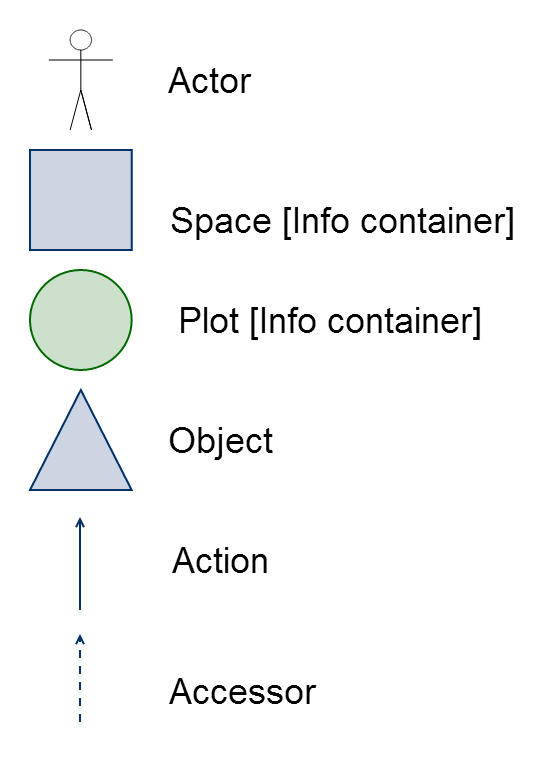
\includegraphics[scale=.3]{symbols}
	\caption{DML Symbols}
	\label{fig:DMLSymbols}	
\end{figure}
\section{Entities}
\diage entities come in four forms; \code{Actors}, \code{Objects}, \code{Spaces} and \code{Events}. The latter two are also information containers which I will discuss in section~\ref{sec:informationcontainers}. The following section will only cover the pure entities; the objects and actors. In conjunction with \code{actions} and \code{accessors} these entities convey story information and plot progression. 
\subsection{Objects}
\diage objects form the basis of all entities. They represent the props and items that we find in the world that have narrative importance. For example; if the Player walks in to a shop \diage does not specify all items that one could buy in the shop, but only those that have plot importance. In terms, these objects should adhere to the \textit{Checkhov's Gun} principle. This dramatic principle states that all objects used in a narrative should eventually be used. I quote: "\textit{One must never place a loaded rifle on the stage if it isn't going to go off. It's wrong to make promises you don't mean to keep.\footnote{\url{http://berlin.wolf.ox.ac.uk/lists/quotations/quotations_by_ib.html}}}"
Objects have three properties; a \code{name}, a \code{ID} and a \code{type} The ID is a unique identifier dependant on the type. And the type is used with actions/accessors as seen in figure~\ref{fig:actions} (Futher discussed in section~\ref{sec:actors}). The name is the noun given to an object within the story context. For example; The player receives the \textit{Skeleton Key of Awesomeness}, but the type is just \code{key} giving it no special properties than any other key. It might make sense to name an object something else than it's type, but a name is not given it defaults to it's type. 
Objects form the world, and all other entities derive from the \diage object. This means that all entities have the same properties as the object, but can extend upon it.
\subsection{Actors}
\label{sec:actors}
An actor is the representation of any one object that can, as the noun implies, act. Examples are the store-clerk, a wandering adventurer or the player. The actor is the only entity that can physically interact with the world, and by doing so the only that can change the world's state. By being able to change the world, the actors are the only entities that can ensure plot progression. 
Just like the object, an actor has three properties; a \code{name}, a \code{ID} and a \code{type}. The type property is used in predefined actions as seen in figure~\ref{fig:actions:npc}. This figure defines that the \code{Player} can \textbf{speak} to all actors of type \code{NPC}. A further glance at figure~\ref{fig:actions} shows some more actions that could be defined for the player actor. These predefined actions tell us that the player can trigger all events and enter all spaces. I will expand upon these actions in section~\ref{sec:actions_and_accessors}.

\section{Information Containers}
\label{sec:informationcontainers}
Information containers are entities that hold story information. A space holds information about it's spacial children, and events release information into spaces when they are resolved. Information containers have the unique property that they are nestable. For example; a space that represents a city can hold several spaces that represents housing. 

\subsection{Spaces}
A space is the representation of any segment of the world or the world itself. As spaces are info containers they are nestable, as mentioned before, but they differ in the fact that they can hold every entity as a child. These children make up the spacial awareness of the space and tells us what information it can pas on to actors. Usually an actor gains all the information a space can give upon the moment it enters the space; when the actor becomes a child object to the space. This can be modified, and some parts of information maybe withheld from the actor, but this is where the events come in.

\subsection{Events}
A event is the odd one out as an entity, as it is the only one that does not represent something within the narrative. A event is the abstraction of information that is released into the story when an actor - usually the player - interacts with it, thus events are used for story pacing and narrative convenience. When we need the state of a space to change we use a event to initiate that change. This only applies on the narrative context of the world, because \diage does not specify everything that happens with in the interactive context. For example; if the player went to a store to buy some cheese to eat. \diage only specifies the store's loss of the cheese, if said food item is a special narrative item. Like a poisonous piece of cheese that the villain left there as a cunning trap for our hero. Events make the world go round and are the dynamic forces in \diage.

\section{Actions and Accessors}
\label{sec:actions_and_accessors}
Actions and accessors are the abstract connectors in \diage. They convey what actors can do (actions) and what knowledge they possess (accessors). Some accessors are implied, due to the fact that an actor might be the child of a space, in other cases these connections are explicitly added to a \diage model. If we review the diagram in figure~\ref{fig:examplediagram} we see that the mayor has no connections whatsoever. This would imply that the Mayor has no knowledge about what's or who's in the store. If we compare that figure to figure~\ref{fig:example:accessors}, we see that the Mayor now has a connection to the Shop, thus we can be sure that the Mayor has the knowledge it would have, if it had been in the shop space itself.

\begin{figure}[ht]
	\centering
	\begin{subfigure}[b]{0.3\textwidth}
		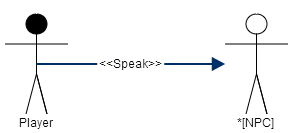
\includegraphics[width=\textwidth]{npc_action}
		\caption{A standard action for NPC interaction}\label{fig:actions:npc}
	\end{subfigure}
	\begin{subfigure}[b]{0.3\textwidth}
		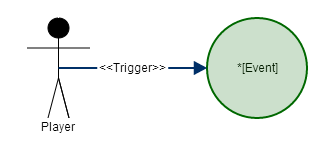
\includegraphics[width=\textwidth]{event_action}
		\caption{A standard action for event interaction}\label{fig:actions:event}
	\end{subfigure}
	\begin{subfigure}[b]{0.3\textwidth}
		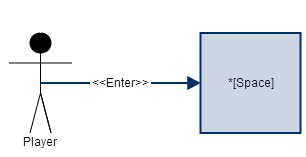
\includegraphics[width=\textwidth]{space_action}
		\caption{A standard action for space interaction}\label{fig:actions:space}
	\end{subfigure}
	\caption{Predefined actions}\label{fig:actions}
\end{figure}

\begin{figure}[ht]
	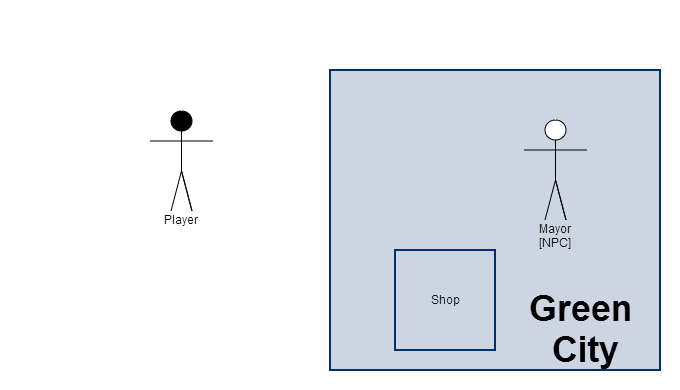
\includegraphics[scale=.5]{diagram_actor_example}
	\caption{An example of a Diage diagram using predefined actions}\label{fig:examplediagram}
\end{figure}
\begin{figure}
	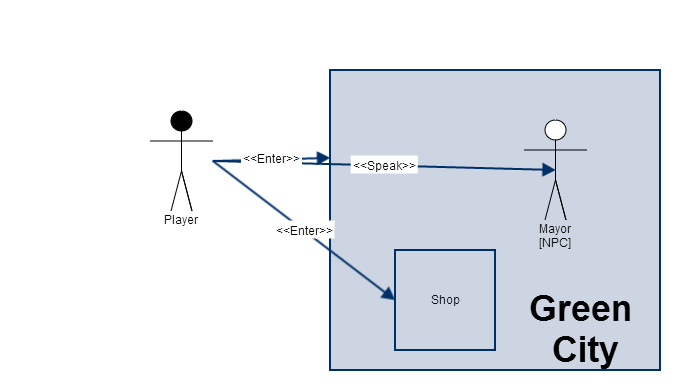
\includegraphics[scale=.5]{diagram_actor_example_verbose}
	\caption{An example of a Diage diagram without using predefined actions}\label{fig:examplediagramverbose}
\end{figure}
\begin{figure}
	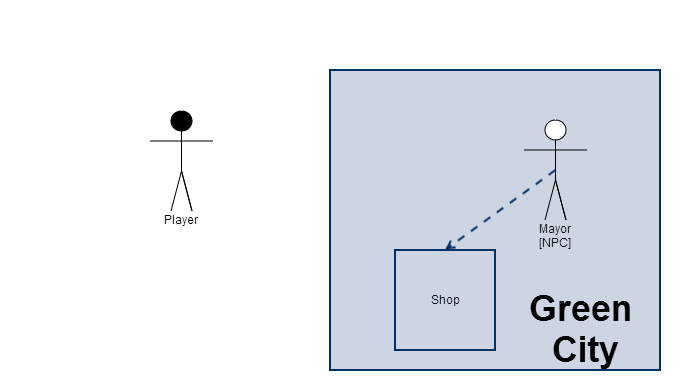
\includegraphics[scale=.5]{diagram_accessor_example}
	\caption{A \diage diagram showing a explicit connection between the Mayor and the Shop}
	\label{fig:example:accessors}
\end{figure}
\section{Diage as a graph}
Diage can be defined by DML, but also as a graph. This form of representation allows us to use graph theory to manipulate and transform the diagram, which we'll cover in the next chapter\footnote{SHOULD BE LEFT FOR FINAL!}

\begin{figure}
	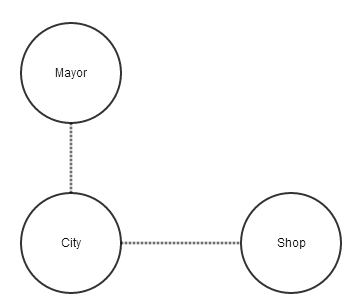
\includegraphics[scale=.5]{diagram_graph}
	\caption{Figure~\ref{fig:examplediagram} as a graph}\label{fig:example:graph}
\end{figure}
\chapter{Narrative planning}
\textit{This chapter will discuss the use of a narrative planner as used by many of my sources. I want to incorporate a narrative planner that smartly uses \diage to manipulate a narrative and conveys that in a way we petty humans can understand}
\\\\
A lot of related work as gone into the use of a planning system that decides on the narrative structure. Researchers like Riedl~\cite{Riedl03character-focusednarrative}\cite{Riedl:2003:MIU:860575.860694}\cite{Riedl:2004:IPM:1018409.1018753} and Cavazza~\cite{Cavazza:2002:CIS:630325.630747} have been researching the use of artificial intelligence for years, and have made some interesting planning systems like \textit{Memesis}~\citationneeded. I am developing my own planning system to use \diage as input and output and use \textit{Ludoscope} to manipulate the diagram as a graph (see section~\ref{sec:ludoscope} for more on Ludoscope) for the model transformations. 
\chapter{Usage in Ludoscope}
\label{sec:ludoscope}
\textit{This chapter will discuss the usage of Ludoscope for the procedural generation of plots and the diage knowledge model for a hypothetical quest generator.}
\chapter{Further study}
\label{sec:further_study}
\bibliographystyle{plain}
\bibliography{diage}
\end{document}